\begin{center}
	\begin{tabular}{M{9.25cm}M{8.75cm}}
		\textbf{TRƯỜNG THCS-THPT NGUYỄN KHUYẾN}& \textbf{ÔN TẬP KIỂM TRA CUỐI HỌC KÌ II}\\
		\textbf{MÃ ĐỀ: 002}& \textbf{Bài thi môn: VẬT LÝ 10}\\
		\textit{(Đề thi có 04 trang)}& \textit{Thời gian làm bài: 45 phút, không kể phát đề}
		
		\noindent\rule{4cm}{0.8pt} \\
	\end{tabular}
\end{center}
\setcounter{section}{0}
\section{Câu trắc nghiệm nhiều phương án lựa chọn}
\textit{Thí sinh trả lời từ câu 1 đến câu 12. Mỗi câu hỏi thí sinh chọn một phương án}
\setcounter{ex}{0}
\Opensolutionfile{ans}[ans/D10-CK2-002-TN]
% ===================================================================
\begin{ex}
	Trong trò chơi trượt nước, người chơi phải đi cầu thang lên đến đỉnh của đường trượt nước ở một độ cao nhất định nào đó so với mặt đất. Sau đó, người chơi dùng ván để trượt từ trên cao xuống. Khi đang  trượt xuống thì
	\choice
	{cơ năng của người chơi tăng lên, động năng và thế năng không đổi}
	{động năng của người chơi tăng lên và cơ năng của học giảm}
	{động năng của người chơi đã chuyển hóa thành thế năng của họ}
	{\True thế năng của người chơi đã chuyển hóa thành động năng của họ}
	\loigiai{}
\end{ex}
% ===================================================================
\begin{ex}
	Trong các hình vẽ dưới đây, hình vẽ nào biểu diễn đúng vector độ biến thiên động lượng $\Delta\vec{p}=\vec{p}_2-\vec{p}_1$?
	\choice
	{\begin{tikzpicture}
			\coordinate (O) at(0,0);
			\coordinate (A) at(3,0);
			\coordinate (B) at(2,1.5);
			\draw[-stealth, line width=1.5pt, blue] (O)--(A);
			\draw[-stealth, line width=1.5pt, blue] (O)--(B);
			\draw[-stealth, line width=1.5pt, blue] (A)--(B);
			\node[below, blue] at ($(O)!0.5!(A)$) {$\vec{p}_2$};
			\node[above left, blue] at ($(O)!0.5!(B)$) {$\vec{p}_1$};
			\node[right, blue] at ($(A)!0.5!(B)$) {$\Delta\vec{p}$};
	\end{tikzpicture}}
	{\begin{tikzpicture}
			\coordinate (O) at(0,0);
			\coordinate (A) at(3,0);
			\coordinate (B) at(-2,2);
			\coordinate (C) at (1,2);
			\draw[-stealth, line width=1.5pt, blue] (O)--(A);
			\draw[-stealth, line width=1.5pt, blue] (O)--(B);
			\draw[-stealth, line width=1.5pt, blue] (O)--(C);
			\draw[dashed, line width=1pt] (B)--(C)--(A);
			\node[below, blue] at ($(O)!0.5!(A)$) {$\vec{p}_2$};
			\node[left, blue] at ($(O)!0.5!(B)$) {$\vec{p}_1$};
			\node[left, blue] at ($(O)!0.5!(C)$) {$\Delta\vec{p}$};
	\end{tikzpicture}}
	{\begin{tikzpicture}
			\coordinate (O) at(0,0);
			\coordinate (A) at(3,0);
			\coordinate (B) at(0,0.5);
			\coordinate (C) at(2,0.5);
			\coordinate (D) at(3,0.5);
			\draw[-stealth, line width=1.5pt, blue] (O)--(A);
			\draw[-stealth, line width=1.5pt, blue] (B)--(C);
			\draw[-stealth, line width=1.5pt, blue] (D)--(C);
			\node[below, blue] at ($(O)!0.5!(A)$) {$\vec{p}_2$};
			\node[above left, blue] at ($(C)!0.5!(B)$) {$\vec{p}_1$};
			\node[above, blue] at ($(C)!0.5!(D)$) {$\Delta\vec{p}$};
	\end{tikzpicture}}
	{\True \begin{tikzpicture}
			\coordinate (O) at(0,0);
			\coordinate (A) at(3,0);
			\coordinate (B) at(-2,-1.5);
			\draw[-stealth, line width=1.5pt, blue] (O)--(A);
			\draw[-stealth, line width=1.5pt, blue] (O)--(B);
			\draw[-stealth, line width=1.5pt, blue] ($(B)+(0,-0.1)$)--($(A)+(0,-0.1)$);
			\node[above, blue] at ($(O)!0.5!(A)$) {$\vec{p}_2$};
			\node[above left, blue] at ($(O)!0.5!(B)$) {$\vec{p}_1$};
			\node[below right, blue] at ($(A)!0.5!(B)$) {$\Delta\vec{p}$};
	\end{tikzpicture}}
	\loigiai{}
\end{ex}
% ===================================================================
\begin{ex}
	Một quả bóng khối lượng \SI{0.5}{\kilogram} đang nằm yên thì được đá cho nó chuyển động với vận tốc \SI{40}{\meter/\second}. Xung lượng của lực tác dụng lên quả bóng bằng
	\choice
	{\SI{80}{\newton\cdot\second}}
	{\SI{8}{\newton\cdot\second}}
	{\True \SI{20}{\newton\cdot\second}}
	{\SI{45}{\newton\cdot\second}}
	\loigiai{}
\end{ex}
% ===================================================================
\begin{ex}
	Một người dùng dây, kéo một thùng hàng nằm trên mặt đất theo hướng hợp với phương ngang một góc \SI{30}{\degree}. Biết lực kéo $\vec{F}$ có độ lớn là \SI{15}{\newton}. Công của lực $\vec{F}$ khi vật dịch chuyển được \SI{3}{\meter} là
	\choice
	{\SI{10}{\joule}}
	{\SI{45}{\joule}}
	{$\xsi{30\sqrt{3}}{\joule}$}
	{\True $\xsi{22,5\sqrt{3}}{\joule}$}
	\loigiai{}
\end{ex}

% ===================================================================
\begin{ex}
	Viên đạn khối lượng \SI{20}{\gram} đang bay với vận tốc \SI{600}{\meter/\second} thì gặp một cánh cửa thép. Đạn xuyên qua cửa trong thời gian \SI{0.002}{\second}. Sau khi xuyên qua cánh cửa vận tốc của đạn còn \SI{300}{\meter/\second}. Lực cản trung bình của cửa tác dụng lên đạn có độ lớn bằng
	\choice
	{\True \SI{3000}{\newton}}
	{\SI{900}{\newton}}
	{\SI{9000}{\newton}}
	{\SI{30000}{\newton}}
	\loigiai{}
\end{ex}
% ===================================================================
\begin{ex}
	Muốn bơm nước từ một giếng sâu \SI{15}{\meter} lên mặt đất người ta dùng một máy bơm có công suất \SI{2}{CV} (mã lực), hiệu suất \SI{50}{\percent}. Tính lượng nước bơm được trong 1 giờ. Cho biết $\SI{1}{CV}=\SI{736}{\watt}$. Lấy $g=\SI{10}{\meter/\second^2}$ và khối lượng riêng của nước là \SI{1000}{\kilogram/\meter^3}.
	\choice
	{\True \SI{17.664}{\meter^3}}
	{\SI{8.832}{\meter^3}}
	{\SI{35.328}{\meter^3}}
	{\SI{70.656}{\meter^3}}
	\loigiai{}
\end{ex}
% ===================================================================
\begin{ex}
	
	\immini{Trên hình bên là đồ thị độ dịch chuyển - thời gian của một vật có khối lượng \SI{3}{\kilogram}. Động lượng của vật tại thời điểm $t_1=\SI{1}{\second}$ và thời điểm $t_2=\SI{5}{\second}$ lần lượt bằng\choice
		{\True $p_1=\SI{4}{\kilogram\cdot\meter/\second}$ và $p_2=0$}
		{$p_1=0$ và $p_2=0$}
		{$p_1=0$ và $p_2=\SI{-4}{\kilogram\cdot\meter/\second}$}
		{$p_1=\SI{4}{\kilogram\cdot\meter/\second}$ và $p_2=\SI{-4}{\kilogram\cdot\meter/\second}$}}
	{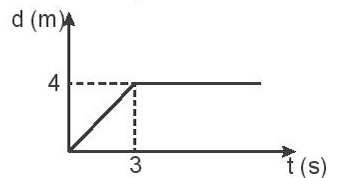
\includegraphics[scale=0.5]{../figs/D10-CK2-001-2}}
	\loigiai{}
\end{ex}
% ===================================================================
\begin{ex}
	Hai viên bi có khối lượng \SI{200}{\gram} và \SI{300}{\gram}, chuyển động trên mặt phẳng ngang không ma sát với tốc độ lần lượt là \SI{8}{\meter/\second}  và \SI{5}{\meter/\second} theo hai phương vuông góc với nhau. Tổng động lượng của hệ hai viên bi \textbf{gần nhất} giá trị nào dưới đây?
	\choice
	{\SI{2.7}{\kilogram\cdot\meter/\second}}
	{\SI{0.1}{\kilogram\cdot\meter/\second}}
	{\True \SI{2.2}{\kilogram\cdot\meter/\second}}
	{\SI{3.1}{\kilogram\cdot\meter/\second}}
	\loigiai{}
\end{ex}
% ===================================================================
\begin{ex}
	Một khẩu đại bác có khối lượng 4 tấn, bắn đi một viên đạn theo phương ngang có khối lượng \SI{10}{\kilogram} với vận tốc \SI{400}{\meter/\second}. Coi như lúc đầu, hệ đại bác và đạn đứng yên. Tốc độ giật lùi của đại bác ngay sau đó bằng
	\choice
	{\SI{3}{\meter/\second}}
	{\SI{2}{\meter/\second}}
	{\SI{4}{\meter/\second}}
	{\True \SI{1}{\meter/\second}}
	\loigiai{}
\end{ex}
% ===================================================================
\begin{ex}
	Một chiếc xe đạp chạy với tốc độ $\SI{40}{\kilo\meter/\hour}$ trên một vòng đua có bán kính \SI{100}{\meter}. Độ lớn gia tốc hướng tâm của xe bằng
	\choice
	{\SI{0.11}{\meter/\second^2}}
	{\SI{0.4}{\meter/\second^2}}
	{\True \SI{1.23}{\meter/\second^2}}
	{\SI{16}{\meter/\second^2}}
	\loigiai{}
\end{ex}
% ===================================================================
\begin{ex}
	Hai điểm A và B trên cùng một bán kính của một vô lăng đang quay đều, cách nhau \SI{20}{\centi\meter}. Điểm A ở phía ngoài có tốc độ $v_{\mathrm{A}}=\SI{0.6}{\meter/\second}$, còn điểm B có $v_{\mathrm{B}}=\SI{0.2}{\meter/\second}$. Tốc độ góc của vô lăng và khoảng cách từ điểm B đến trục quay là
	\choice
	{\True \SI{2}{\radian/\second}; \SI{10}{\centi\meter}}
	{\SI{3}{\radian/\second}; \SI{30}{\centi\meter}}
	{\SI{1}{\radian/\second}; \SI{20}{\centi\meter}}
	{\SI{4}{\radian/\second}; \SI{40}{\centi\meter}}
	\loigiai{}
\end{ex}
% ===================================================================
\begin{ex}
	Hai viên bi giống hệt nhau tiếp xúc với nhau và nằm trên mặt bàn không có ma sát thi bị một viên bi khác có cùng khối lượng đang chuyển động với vận tốc $v$ theo đường thẳng qua tâm của hai viên bi tới va chạm. Nếu va chạm là tuyệt đối đàn hồi, thì hình nào sau đây là kết quả có thể xảy ra sau va chạm?
	\choice
	{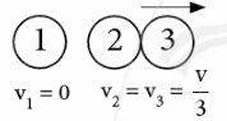
\includegraphics[scale=0.6]{../figs/D10-CK2-001-1a}}
	{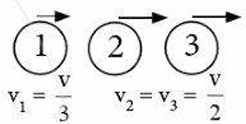
\includegraphics[scale=0.6]{../figs/D10-CK2-001-1b}}
	{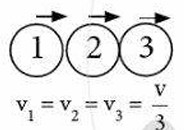
\includegraphics[scale=0.6]{../figs/D10-CK2-001-1c}}
	{\True 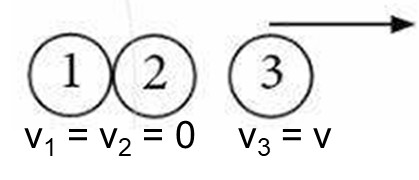
\includegraphics[scale=0.6]{../figs/D10-CK2-001-1d}}
	\loigiai{}
\end{ex}
\Closesolutionfile{ans}
\section{Câu trắc nghiệm đúng/sai} 
\textit{Thí sinh trả lời từ câu 1 đến câu 4. Trong mỗi ý \textbf{a)}, \textbf{b)}, \textbf{c)}, \textbf{d)} ở mỗi câu, thí sinh chọn đúng hoặc sai}
\setcounter{ex}{0}\\
\Opensolutionfile{ans}[ans/D10-CK2-002-TF]
% ===================================================================
\begin{ex}
	Tại điểm A cách mặt đất \SI{4}{\meter} một vật có khối lượng \SI{2}{\kilogram} được ném thẳng đứng lên trên với tốc độ đầu \SI{10}{\meter/\second}. Chọn mốc thế năng tại mặt đất. Bỏ qua lực cản của không khí. Lấy $g=\SI{10}{\meter/\second^2}$.
	
	\choiceTF
	{Động năng của vật tại điểm A có giá trị \SI{180}{\joule}}
	{Thế năng của vật tại điểm A đạt giá trị cực đại}
	{\True Thế năng của vật tại vị trí cách mặt đất \SI{2}{\meter} là \SI{40}{\joule}}
	{\True Độ cao cực đại mà vật đạt được là \SI{9}{\meter}}
	\loigiai{}
\end{ex}
% ===================================================================
\begin{ex}
	\immini{Hình bên cạnh là phương án bố trí thí nghiệm kiểm chứng định luật bảo toàn động lượng cho trường hợp hai vật va chạm đàn hồi.
		Hai vật đặt trên đệm khí, giữa hai vật có một lò xo bị nén. Dùng sợi dây buộc giữ hai vật với nhau. Khi đốt sợi dây, hai lò xo giãn ra, hai vật bị đẩy về phía hai cổng quang điện.}
	{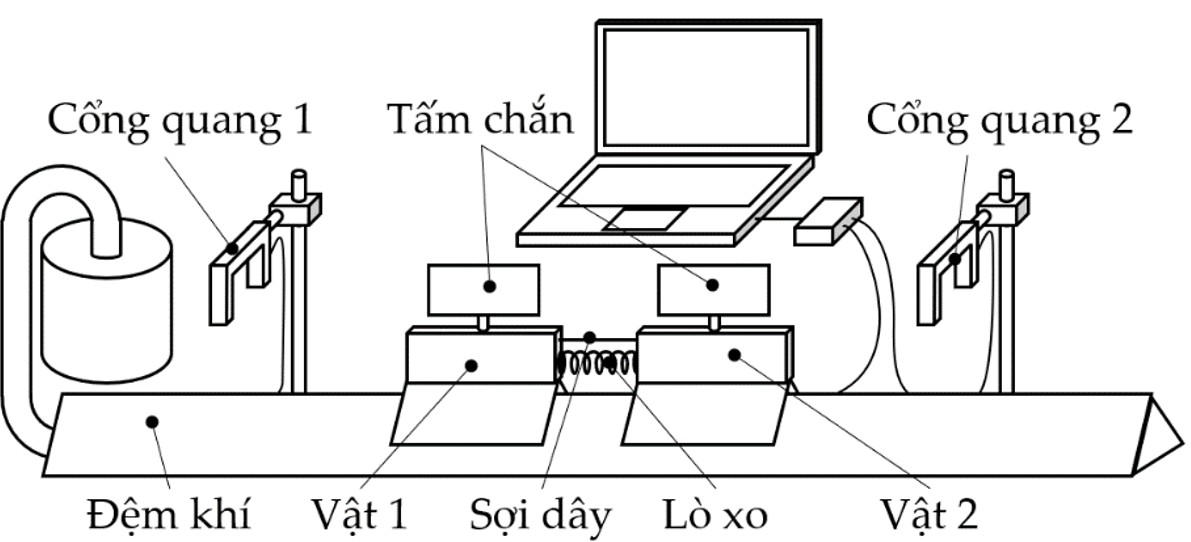
\includegraphics[scale=0.3]{../figs/D10-CK2-002-2}}
	\choiceTF
	{Hệ hai vật trong thí nghiệm trên được xem là hệ kín vì không có ngoại lực tác dụng lên hệ}
	{\True Nếu độ dài tấm chắn trên hai vật lần lượt là $d_1$ và $d_2$, thời gian các tấm chắn che hai cổng quang lần lượt là $t_1$ và $t_2$ thì tốc độ của hai vật sau khi cắt dây là $v_1=d_1/t_1$ và $v_2=d_2/t_2$}
	{Động lượng của hệ hai xe trước khi cắt dây là $\left(m_1+m_2\right)\cdot\left(\dfrac{v_1+v_2}{2}\right)$}
	{\True Định luật bảo toàn động lượng được kiểm chứng nếu $m_1v_1=m_2v_2$}
	\loigiai{}
\end{ex}
% ===================================================================
\begin{ex}
	Hình bên mô tả cấu tạo bộ phận truyền động trong một chiếc xe đạp. Khi chúng ta thao tác đạp lên bàn đạp, lực đạp được truyền từ bàn đạp dến giò đĩa là đĩa xích quay. Sự quay của đĩa xích làm dây xích chuyển động kéo líp cùng bánh sau quay theo.  Xét cơ cấu truyền động trong một xe đạp với đĩa xích và líp có đường kính lần lượt là $d_1$ và $d_2$ như hình bên. Đĩa xích quay với tốc độ góc $n_1$ và líp quay với tốc độ góc $n_2$.
	\begin{center}
		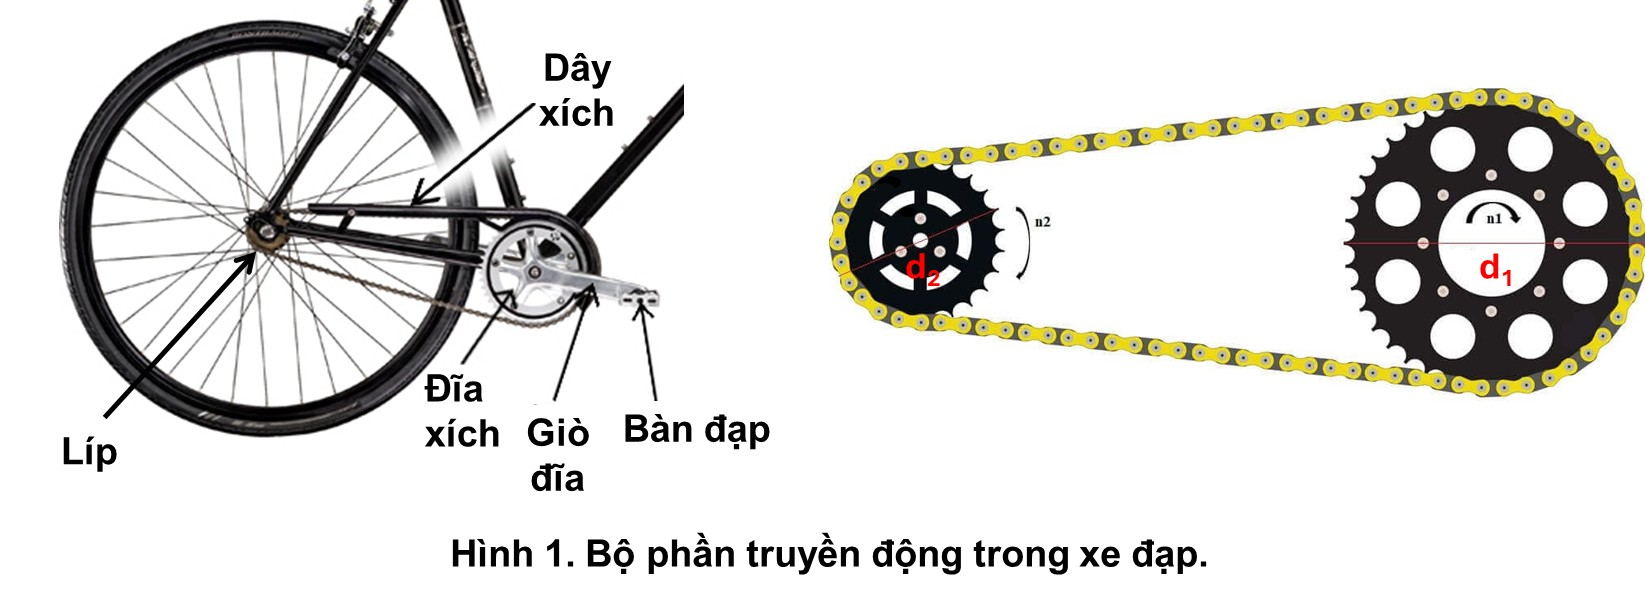
\includegraphics[scale=0.5]{../figs/D10-CK2-002-3}
	\end{center}
	\choiceTF
	{\True Để đĩa và líp ăn khớp được với nhau thì tỉ số giữa số răng trên đĩa và líp $\dfrac{N_2}{N_1}=\dfrac{d_2}{d_1}$}
	{\True Trong quá trình truyền động, tốc độ góc của đĩa xích và líp liên hệ với nhau $n_1d_1=n_2d_2$}
	{\True Gia tốc hướng tâm tại một điểm trên vành líp lớn hơn gia tốc hướng tâm tại một điểm trên vành đĩa xích}
	{\True Đường kính bánh xe đạp là \SI{66}{\centi\meter}. Nếu xe chạy được quãng đường \SI{10}{\kilo\meter} thì líp xe đã quay được 4823 vòng}
	\loigiai{}
\end{ex}
% ===================================================================
\begin{ex}
	\immini{Một trạm vũ trụ chuyển động đều quanh Trái Đất trên một quỹ đạo tròn ở độ cao $h=\SI{400}{\kilo\meter}$ so với mặt đất. Trên mặt đất, trong mặt phẳng quỹ đạo của trạm vũ trụ, người ta quan sát thấy trạm vũ trụ như là một điểm sáng nhỏ di chuyển trên bầu trời. Giả sử bỏ qua chuyển động tự quay của Trái Đất quanh trục. Gia tốc trọng trường tại vị trí của trạm vũ trụ đóng vai trò là gia tốc hướng tâm và được xác định bởi biểu thức $g=g_0\cdot\left(\dfrac{R}{R+h}\right)^2$, với $g_0=\SI{9.81}{\meter/\second^2}$ là gia tốc rơi tự do tại bề mặt của Trái Đất và $R=\SI{6370}{\kilo\meter}$ là bán kính Trái Đất.}
	{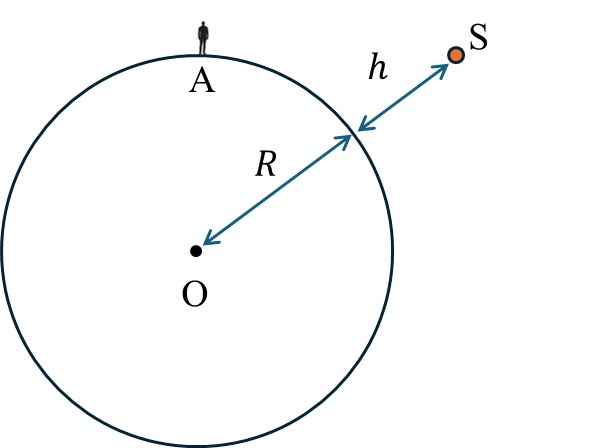
\includegraphics[scale=0.5]{../figs/D10-CK2-002-1}}
	\choiceTF
	{\True Gia tốc hướng tâm của trạm vũ trụ có độ lớn xấp xỉ \SI{8.69}{\meter/\second^2}}
	{Thời gian để trạm hoàn thành 1 vòng quay quanh Trái Đất là 1 giờ 29 phút}
	{\True Tốc độ chuyển động của trạm vũ trụ xấp xỉ \SI{27605}{\kilo\meter/\hour}}
	{\True Người quan sát tại A sẽ thấy trạm vũ trụ trên bầu trời trong khoảng thời gian 10 phút 10 giây}
	\loigiai{}
\end{ex}

\Closesolutionfile{ans}
\section{Tự luận} 
\setcounter{ex}{0}
\Opensolutionfile{ans}[ans/D10-CK2-002-TL]
% ===============================================================
\begin{ex}\textit{(0,75 điểm)}
	Biết kim phút của đồng hồ treo tường có chiều dài $\ell=\SI{10.0}{\centi\meter}$.
	\begin{enumerate}[label=\alph*)]
		\item Tính độ dịch chuyển góc và quãng đường đi của điểm đầu kim phút trong khoảng thời gian $t=\SI{15.0}{\minute}$.
		\item Biết tỉ số tốc độ của điểm đầu kim phút và tốc độ của điểm đầu kim giờ là \SI{15.0}{}. Tính chiều dài của kim giờ.
	\end{enumerate}
	\loigiai{
		
	}
\end{ex}
% ===============================================================
\begin{ex}\textit{(0,5 điểm)}
	Một vật có khối lượng $m$ chuyển động với tốc độ \SI{3}{\meter/\second} đến va chạm với một vật có khối lượng $2m$ đang đứng yên. Sau va chạm, hai vật dính vào nhau và chuyển động với cùng tốc độ. Xác định tốc độ của hai vật sau va chạm.
	\loigiai{
		
	}
\end{ex}
% ===============================================================
\begin{ex}\textit{(0,75 điểm)}
	Hình bên biểu diễn giá trị của lực $\vec{F}$ tác dụng lên vật nhỏ khối lượng \SI{1.5}{\kilogram} theo thời gian $t$.
\immini{\begin{enumerate}[label=\alph*)]
		\item Xác định xung lượng của lực tác dụng lên vật trong khoảng thời gian $t=0$ đến $t=\SI{3.0}{\second}$.
		\item Nếu ban đầu vật ở trạng thái nghỉ, xác định tốc độ của vật tại thời điểm $t=\SI{3.0}{\second}$ và $t=\SI{5.0}{\second}$.
\end{enumerate}}
{\vspace{-0.5cm}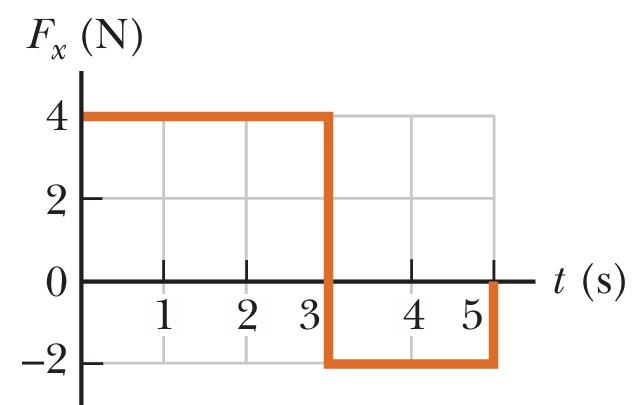
\includegraphics[scale=0.4]{../figs/D10-CK2-002-4}}
	\loigiai{
		
	}
\end{ex}
% ===============================================================
\begin{ex}
Vào năm 1887 tại Bridgeport, Connecticut, C. J. Belknap đã xây dựng máng trượt nước vui chơi như mô hình đơn giản bên dưới. Một người lái trên một chiếc xe trượt nhỏ, có tổng khối lượng \SI{80}{\kilogram}, bắt đầu trượt từ điểm A trên máng với tốc độ \SI{2.5}{\meter/\second}. Máng trượt nghiêng góc $\theta=\SI{10}{\degree}$ và chiều dài $\ell=\SI{54.3}{\meter}$. Khi rời khỏi máng trượt theo phương ngang ở cuối máng (điểm C), người và xe trượt đã lướt trên mặt nước một khoảng $d=\SI{50}{\meter}$ trước khi dừng lại. Bỏ qua ma sát trên máng trượt và lấy $g=\SI{9.81}{\meter/\second^2}$.
\begin{center}
	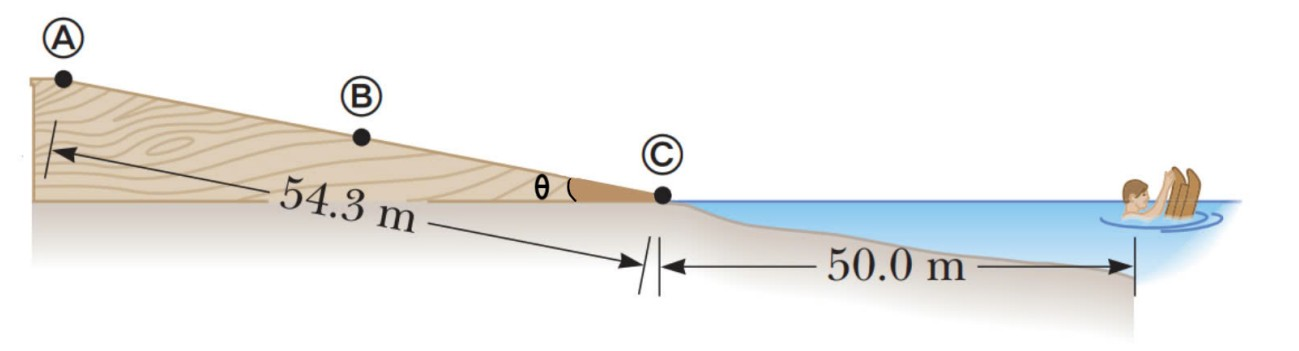
\includegraphics[scale=0.4]{../figs/D10-CK2-002-5}
\end{center}
\begin{enumerate}[label=\alph*)]
	\item Tìm tốc độ của xe trượt tại C.
	\item Cho rằng lực cản của nước tác dụng lên người và xe trượt là không đổi. Tìm độ lớn của lực cản này?
\end{enumerate}
	\loigiai{
		
	}
\end{ex}
\Closesolutionfile{ans}
\begin{center}
	\textbf{--- HẾT ---}
\end{center}